% =====================================================================
% CHAPTER 3: Thiết kế giải thuật
% Pages 31-44 (numbered 15-28)
% Covers the 3-Tier KG-RAG algorithm design
% =====================================================================
\chapter{Thiết kế giải thuật}
\label{chap:thiet-ke-giai-thuat}

Chương này trình bày chi tiết kiến trúc giải thuật 3-Tier KG-RAG được đề xuất,
bao gồm phát biểu bài toán, tổng quan kiến trúc hệ thống, và ba tầng truy xuất:
duyệt cây cấu trúc hướng dẫn bởi LLM, truy xuất ngữ nghĩa hai cấp, và
Reciprocal Rank Fusion với mở rộng Knowledge Graph. Nội dung chương dựa trên
bài báo khoa học đã nộp tại hội nghị SOMET 2026 \cite{le2026threetier}.

% =====================================================================
\section{Phát biểu bài toán}
\label{sec:phat-bieu-bai-toan}

Các văn bản quy phạm Việt Nam thường có cấu trúc phân cấp sáu cấp: Văn bản,
Chương, Mục (nếu có), Điều, Khoản, Điểm với các tham chiếu chéo xuyên suốt giữa
các tài liệu. Truy xuất đoạn văn bản truyền thống coi tài liệu như tập hợp phẳng,
do đó không thể khai thác cấu trúc phân cấp này hoặc thực hiện suy luận đa bước.

Mỗi tài liệu được mô hình hóa dưới dạng cây có gốc (rooted tree), trong đó các
nút tương ứng với các cấp cấu trúc và các cạnh biểu diễn quan hệ cha--con. Toàn
bộ kho tài liệu gồm $m$ văn bản hình thành một Document Forest:

\begin{equation}
  \mathcal{F} = \{T_1, T_2, \ldots, T_m\}
  \label{eq:document-forest}
\end{equation}

\noindent được bổ sung các cạnh tham chiếu chéo liên kết các điều khoản giữa các
cây. Mỗi nút được gán một định danh hợp thành mã hóa vị trí trong cấu trúc phân
cấp, ví dụ \texttt{59-2020-QH14:c2} cho Chương 2, \texttt{59-2020-QH14:d5} cho
Điều 5, cho phép tham chiếu chéo rõ ràng giữa các cây.

\textbf{Bài toán truy xuất:} Cho truy vấn $q$ của người dùng, trả về danh sách
xếp hạng $k$ điều khoản liên quan nhất từ $\mathcal{F}$. Mức chi tiết ở cấp điều
khoản (article-level) là cần thiết vì các quy chế đào tạo tại Việt Nam tổ chức
nội dung theo đơn vị Điều, mỗi Điều quy định một vấn đề cụ thể (ví dụ: Điều 24
quy định điều kiện bảo vệ luận văn, Điều 29 quy định điều kiện tốt nghiệp). Khi
trả lời câu hỏi của học viên, hệ thống cần trích dẫn chính xác đến từng Điều để
đảm bảo tính minh bạch và có thể kiểm chứng, thay vì trả về các đoạn văn bản tùy
ý không rõ nguồn gốc. Yêu cầu này cũng áp dụng tương tự cho miền pháp luật, nơi
các điều khoản luật là đơn vị trích dẫn nhỏ nhất trong thực tiễn tư vấn pháp lý.

% =====================================================================
\section{Tổng quan kiến trúc hệ thống}
\label{sec:tong-quan-kien-truc}

Kiến trúc hệ thống được chia thành hai pha: pha ngoại tuyến (offline phase) và pha
trực tuyến (online phase), như minh họa trong Hình~\ref{fig:kien-truc-he-thong}.

\begin{figure}[htbp]
  \centering
  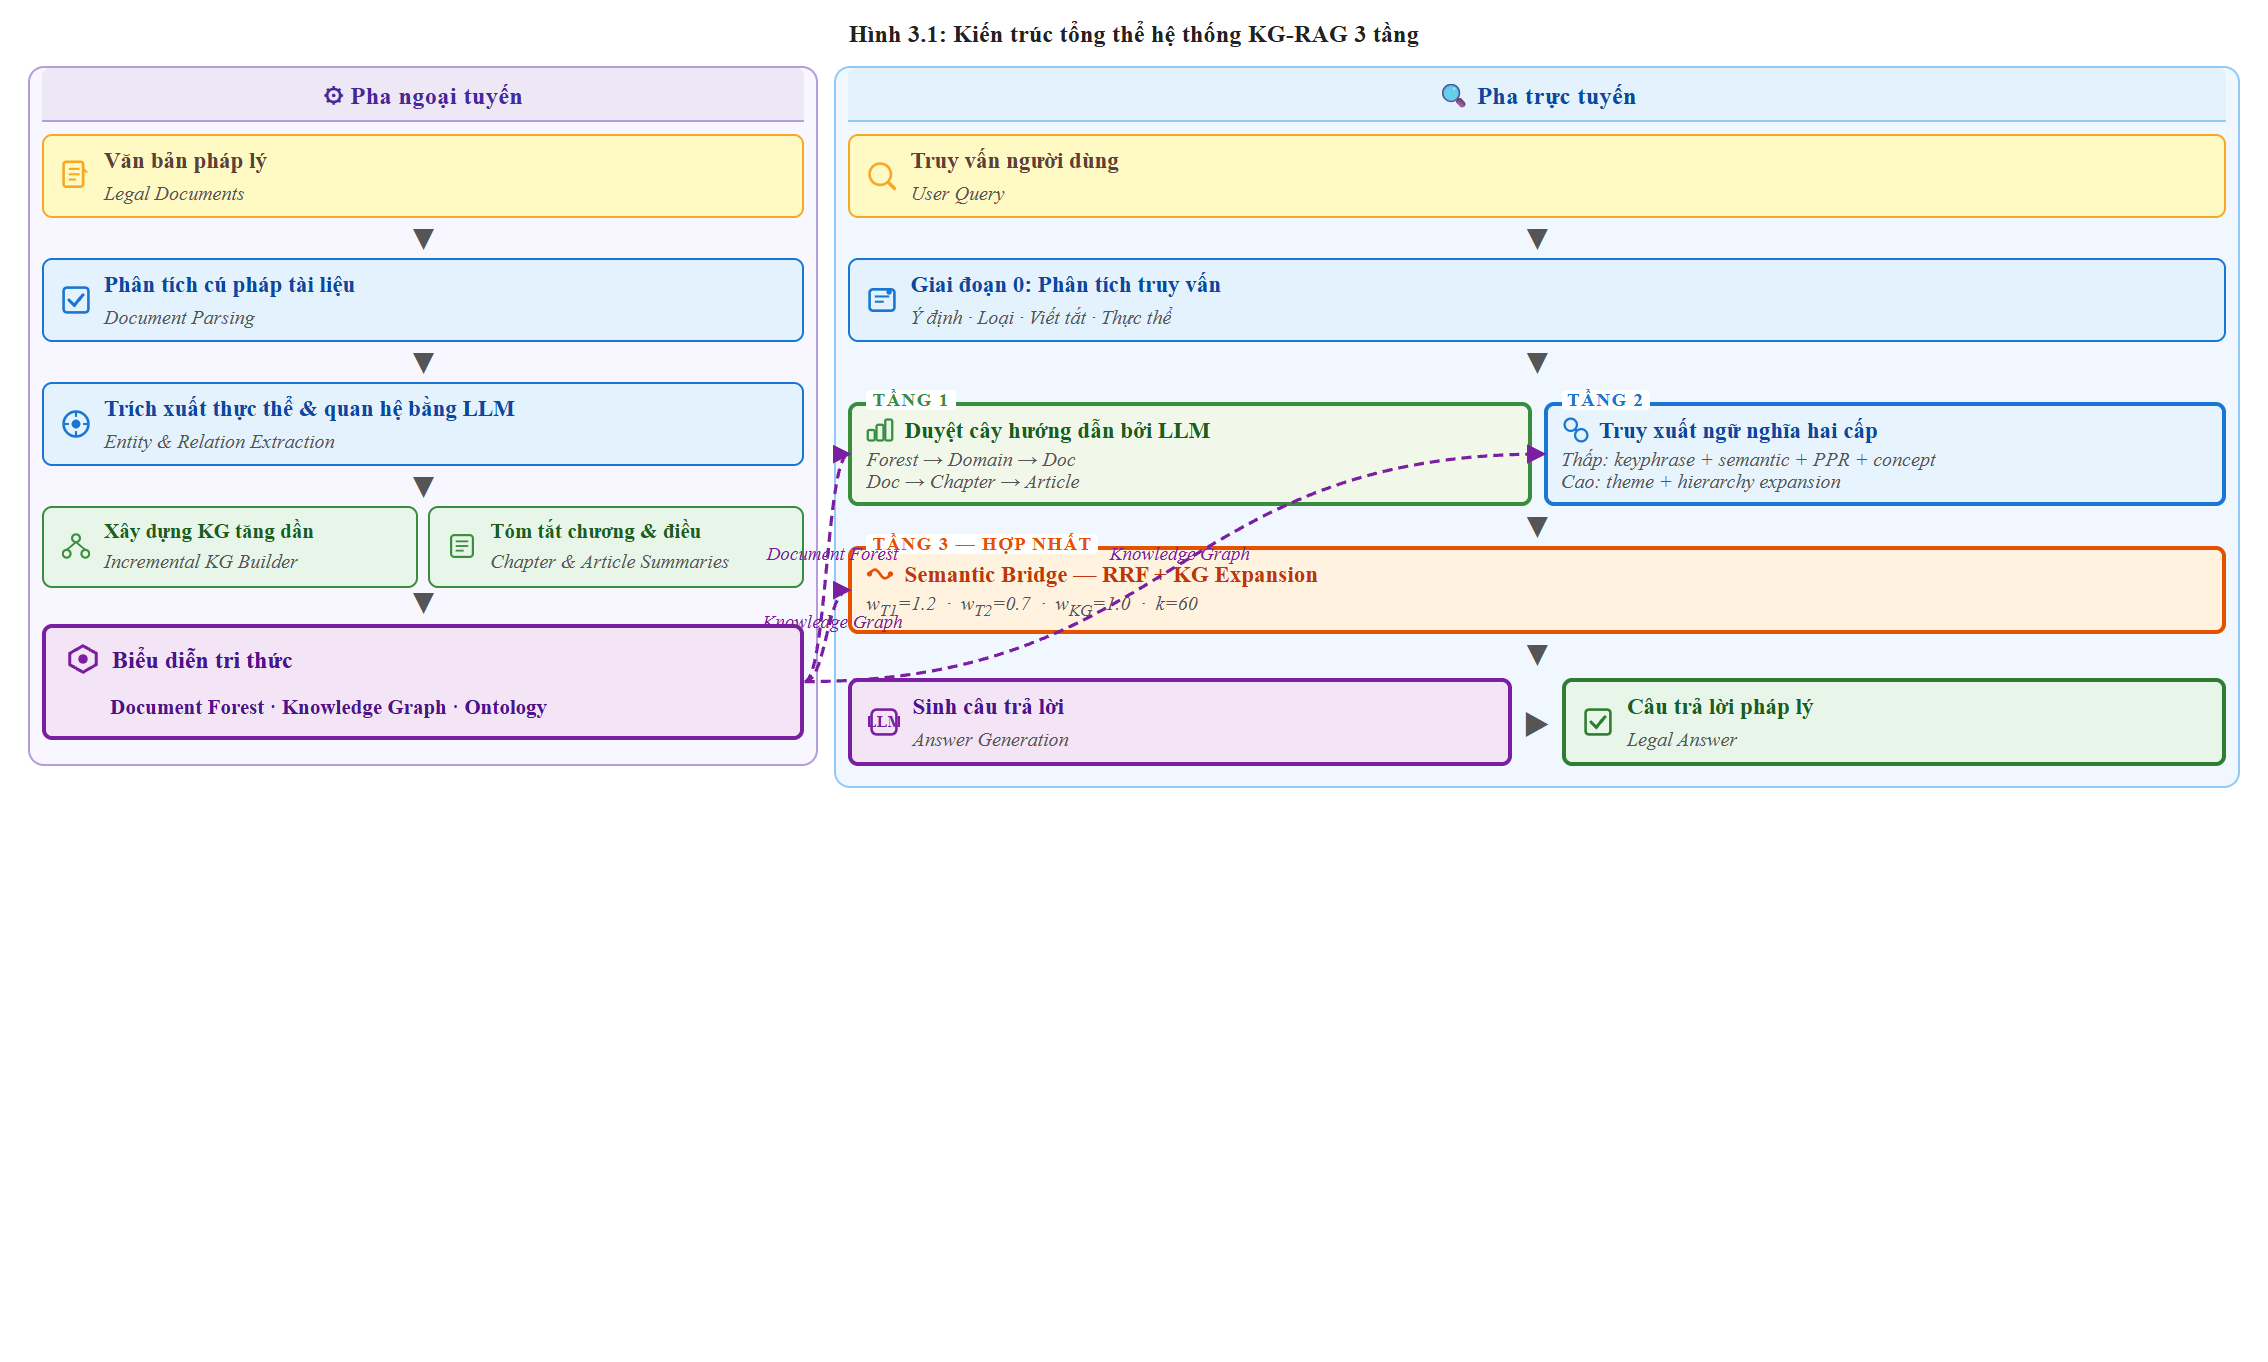
\includegraphics[width=\textwidth]{graphics/figure3-1-system-architecture.png}
  \caption{Kiến trúc hệ thống truy xuất ba tầng. Pha ngoại tuyến (trái): xây dựng
  mô hình tri thức từ văn bản quy phạm. Pha trực tuyến (phải): xử lý truy vấn qua
  Tầng 1 (duyệt cây cấu trúc), Tầng 2 (truy xuất ngữ nghĩa hai cấp), và Tầng 3
  (hợp nhất RRF với mở rộng KG).}
  \label{fig:kien-truc-he-thong}
\end{figure}

% -------------------------------------------------------------------
\subsection{Pha ngoại tuyến}
\label{subsec:pha-ngoai-tuyen}

Pha ngoại tuyến xây dựng bốn bộ biểu diễn tri thức từ kho tài liệu thô, tuân
theo phương pháp kỹ thuật tri thức \cite{sartor2011legalonto}. Các biểu diễn này
phục vụ cho từng tầng truy xuất khác nhau trong pha trực tuyến.

\textbf{Document Forest.}
Mỗi văn bản quy phạm được phân tích thành cây có gốc theo cấu trúc phân cấp
6 cấp: Văn bản $\to$ Chương $\to$ Mục $\to$ Điều $\to$ Khoản $\to$ Điểm. Bộ
phân tích cú pháp (parser) sử dụng regex nhận diện các dấu hiệu phân cấp tiếng
Việt (``Chương I'', ``Điều 5'', ``Khoản 1'', ``Điểm a'') để xây dựng cây cấu
trúc. Mỗi nút trong cây lưu trữ: mã định danh (node\_id), loại nút (node\_type),
tên, nội dung văn bản, và metadata (số hiệu, ngày ban hành, cơ quan ban hành).

Mỗi nút được gán một định danh hợp thành (composite ID) mã hóa vị trí trong cấu
trúc phân cấp theo quy tắc \texttt{\{số\_hiệu\_văn\_bản\}:\{tiền\_tố\}\{số\}}.
Bảng~\ref{tab:node-identifier-rules} trình bày quy tắc đặt tiền tố cho từng cấp.
Ví dụ, Điều 5 của Luật Doanh nghiệp 2020 có định danh \texttt{59-2020-QH14:d5},
Chương 3 của Quy chế 1393 có định danh \texttt{1393-QD-DHQG:c3}. Sơ đồ này cho
phép: tra cứu nút trong thời gian $O(1)$ qua bảng băm, tham chiếu chéo rõ ràng
giữa các cây (ví dụ: \texttt{270-QD-DHCNTT:d24} tham chiếu đến
\texttt{1393-QD-DHQG:d25}), và con người có thể đọc hiểu trực tiếp mà không cần
truy ngược cây.

\begin{table}[htbp]
  \centering
  \caption{Quy tắc đặt định danh nút trong Document Forest}
  \label{tab:node-identifier-rules}
  \begin{tabular}{lll}
    \toprule
    \textbf{Cấp} & \textbf{Tiền tố} & \textbf{Ví dụ} \\
    \midrule
    Văn bản (gốc) & -- & \texttt{59-2020-QH14} \\
    Chương        & \texttt{c} & \texttt{59-2020-QH14:c2} \\
    Mục           & \texttt{s} & \texttt{59-2020-QH14:c2s1} \\
    Điều          & \texttt{d} & \texttt{59-2020-QH14:d5} \\
    Khoản         & \texttt{k} & \texttt{59-2020-QH14:d5k1} \\
    Điểm          & \texttt{p} & \texttt{59-2020-QH14:d5k1pa} \\
    \bottomrule
  \end{tabular}
\end{table}

Tập hợp tất cả các cây tạo thành Document Forest -- cấu trúc dữ liệu trung tâm
cho Tầng 1 (duyệt cây). Các cạnh tham chiếu chéo (cross-reference) được phát hiện
bằng pattern matching trên các chuỗi trích dẫn (ví dụ: ``theo Điều 5 Quy chế
270'', ``căn cứ Khoản 1 Điều 24'') và liên kết các điều khoản giữa các tài liệu
khác nhau. Mỗi tham chiếu được phân loại theo kiểu: THAM\_CHIẾU (dẫn chiếu),
SỬA\_ĐỔI (amend), hoặc THAY\_THẾ (replace).

\textbf{Knowledge Graph.}
Knowledge Graph (KG) được xây dựng qua quy trình bốn bước:

\begin{enumerate}
  \item \textbf{Trích xuất thực thể và quan hệ:} Với mỗi điều khoản, LLM trích
        xuất đồng thời thực thể và quan hệ trong một lời gọi duy nhất (theo phong
        cách LightRAG \cite{guo2025lightrag}). Prompt hướng dẫn LLM trích xuất
        đầy đủ các thực thể quan trọng, ghi evidence (trích dẫn nguyên văn) cho
        mỗi quan hệ, và sử dụng tên thực thể chính xác như trong văn bản (xem Phụ
        lục D, Bảng D.1).

  \item \textbf{Khử trùng lặp thực thể:} Trong quá trình trích xuất, bộ khử trùng
        lặp (deduplicator) sử dụng Jaro-Winkler similarity (ngưỡng $\geq 0{,}98$)
        kết hợp chuẩn hóa dạng chính tắc tiếng Việt (loại dấu, chuẩn hóa viết tắt
        pháp lý) để nhận diện và hợp nhất các thực thể trùng lặp ngay trong quá
        trình xây dựng. Thực thể được hợp nhất lưu giữ tất cả alias, source ID, và
        mô tả dài nhất.

  \item \textbf{Xây dựng ontology:} Hệ thống tự động sinh ontology miền từ dữ
        liệu KG đã trích xuất, sử dụng LLM để phân loại thực thể thành các lớp OWL
        có ý nghĩa. Ontology định nghĩa 14 loại thực thể (Action, Legal Term,
        Organization, Penalty, Condition, Person Role, v.v.) với phân cấp tối đa 4
        cấp. Mỗi lớp có tên tiếng Anh (chuẩn OWL) kèm nhãn và mô tả tiếng Việt.
        Ontology xuất ra định dạng Turtle (.ttl) và JSON.

  \item \textbf{Tinh chỉnh bởi chuyên gia:} Sau khi tự động trích xuất, KG được
        rà soát và tinh chỉnh thủ công bởi chuyên gia miền (expert-in-the-loop).
        Quá trình này bao gồm: thêm các quan hệ bị thiếu (đặc biệt là REFERENCES
        giữa các điều khoản liên quan), xóa các thực thể nhiễu, và điều chỉnh
        trọng số quan hệ (STRONG/WEAK) để cải thiện chất lượng truy xuất.
\end{enumerate}

Bảng~\ref{tab:kg-statistics} tóm tắt thống kê Knowledge Graph được xây dựng. Hệ
thống cũng phân loại quan hệ theo mức độ: quan hệ mạnh (STRONG) gồm references,
requires, depends\_on -- các quan hệ này được sử dụng cho mở rộng KG trong Tầng 3,
trong khi quan hệ yếu (WEAK) như related\_to, is\_a chỉ dùng cho tính điểm ngữ
nghĩa trong Tầng 2.

\begin{table}[htbp]
  \centering
  \caption{Thống kê Knowledge Graph}
  \label{tab:kg-statistics}
  \resizebox{\textwidth}{!}{\begin{tabular}{lrlrlr}
    \toprule
    \textbf{Loại thực thể} & \textbf{Số lượng} &
    \textbf{Loại quan hệ} & \textbf{Số lượng} &
    \textbf{Cấu trúc} & \textbf{Số lượng} \\
    \midrule
    Tổng thực thể  & 5.936 & Tổng quan hệ & 5.963 & Nút          & 9.226 \\
    Action         & 1.903 & requires     & 1.377 & Tài liệu     & 13 \\
    Legal Term     & 1.632 & applies\_to  &   810 & Chương       & 77 \\
    Organization   &   500 & has\_authority &  506 & Điều khoản  & 840 \\
    Legal Reference &  451 & references   &   434 & Tham chiếu chéo & 168 \\
    Khác (9 loại)  & 1.450 & Khác (52 loại) & 2.506 & & \\
    \bottomrule
  \end{tabular}}
\end{table}

\textbf{Tóm tắt chương và điều.}
Để Tầng 1 có thể chọn nhánh mà không cần đọc toàn bộ nội dung điều khoản, hệ
thống sinh tóm tắt cho từng chương và điều bằng LLM. Tóm tắt chương bao gồm phạm
vi điều khoản (ví dụ: ``Điều 1--16'') và danh sách từ khóa đặc trưng do LLM trích
xuất từ nội dung các điều trong chương. Tóm tắt điều gồm tiêu đề và các từ khóa
chính. Các mô tả này được sử dụng trực tiếp làm thuộc tính \texttt{description}
của các nút trong Document Forest, cung cấp đủ ngữ cảnh cho LLM đưa ra quyết định
chọn nhánh trong Loop 1 và Loop 2 (xem prompt chi tiết tại Phụ lục D, Bảng D.2
và D.3).

\textbf{Nhóm miền và cụm chủ đề.}
Hai cấu trúc bổ sung được xây dựng để phục vụ các tầng truy xuất khác nhau:

\begin{itemize}
  \item \textbf{Nhóm miền (Domain Groups):} Các tài liệu được phân nhóm tự động
        dựa trên sự trùng khớp của từ khóa (Jaccard similarity ở mức âm tiết).
        Thuật toán lấy các văn bản gốc làm neo (anchor), sau đó gán các nghị định,
        thông tư liên quan vào nhóm có độ trùng khớp từ khóa cao nhất. Mỗi nhóm
        miền lưu nhãn, danh sách từ khóa đặc trưng, và ID các tài liệu thành viên.
        Cấu trúc này phục vụ Loop 0 của Tầng 1 để nhanh chóng thu hẹp không gian
        tìm kiếm từ toàn bộ kho xuống nhóm miền phù hợp. Để dễ dàng mở rộng sau
        này khi áp dụng phương pháp trên nhiều domain và tài liệu khác nhau hơn.

  \item \textbf{Cụm chủ đề (Theme Clusters):} Các thực thể KG được nhóm thành
        các cụm chủ đề bằng cách phân hoạch đồ thị KG thành các đồ thị con liên
        thông, sau đó sử dụng LLM để trích xuất tên chủ đề, mô tả, và từ khóa tìm
        kiếm cho mỗi cụm. Vector nhúng trung bình của các thực thể trong cụm được
        tính và lưu vào chỉ mục FAISS để phục vụ tìm kiếm ngữ nghĩa nhanh. Cấu
        trúc này phục vụ high-level (theme matching) của Tầng 2.
\end{itemize}

Hình~\ref{fig:offline-pipeline} minh họa toàn bộ quy trình xây dựng tri thức ngoại
tuyến với ba track song song: Document Forest, Knowledge Graph, và các cấu trúc bổ
sung phục vụ từng tầng truy xuất.

\begin{figure}[htbp]
  \centering
  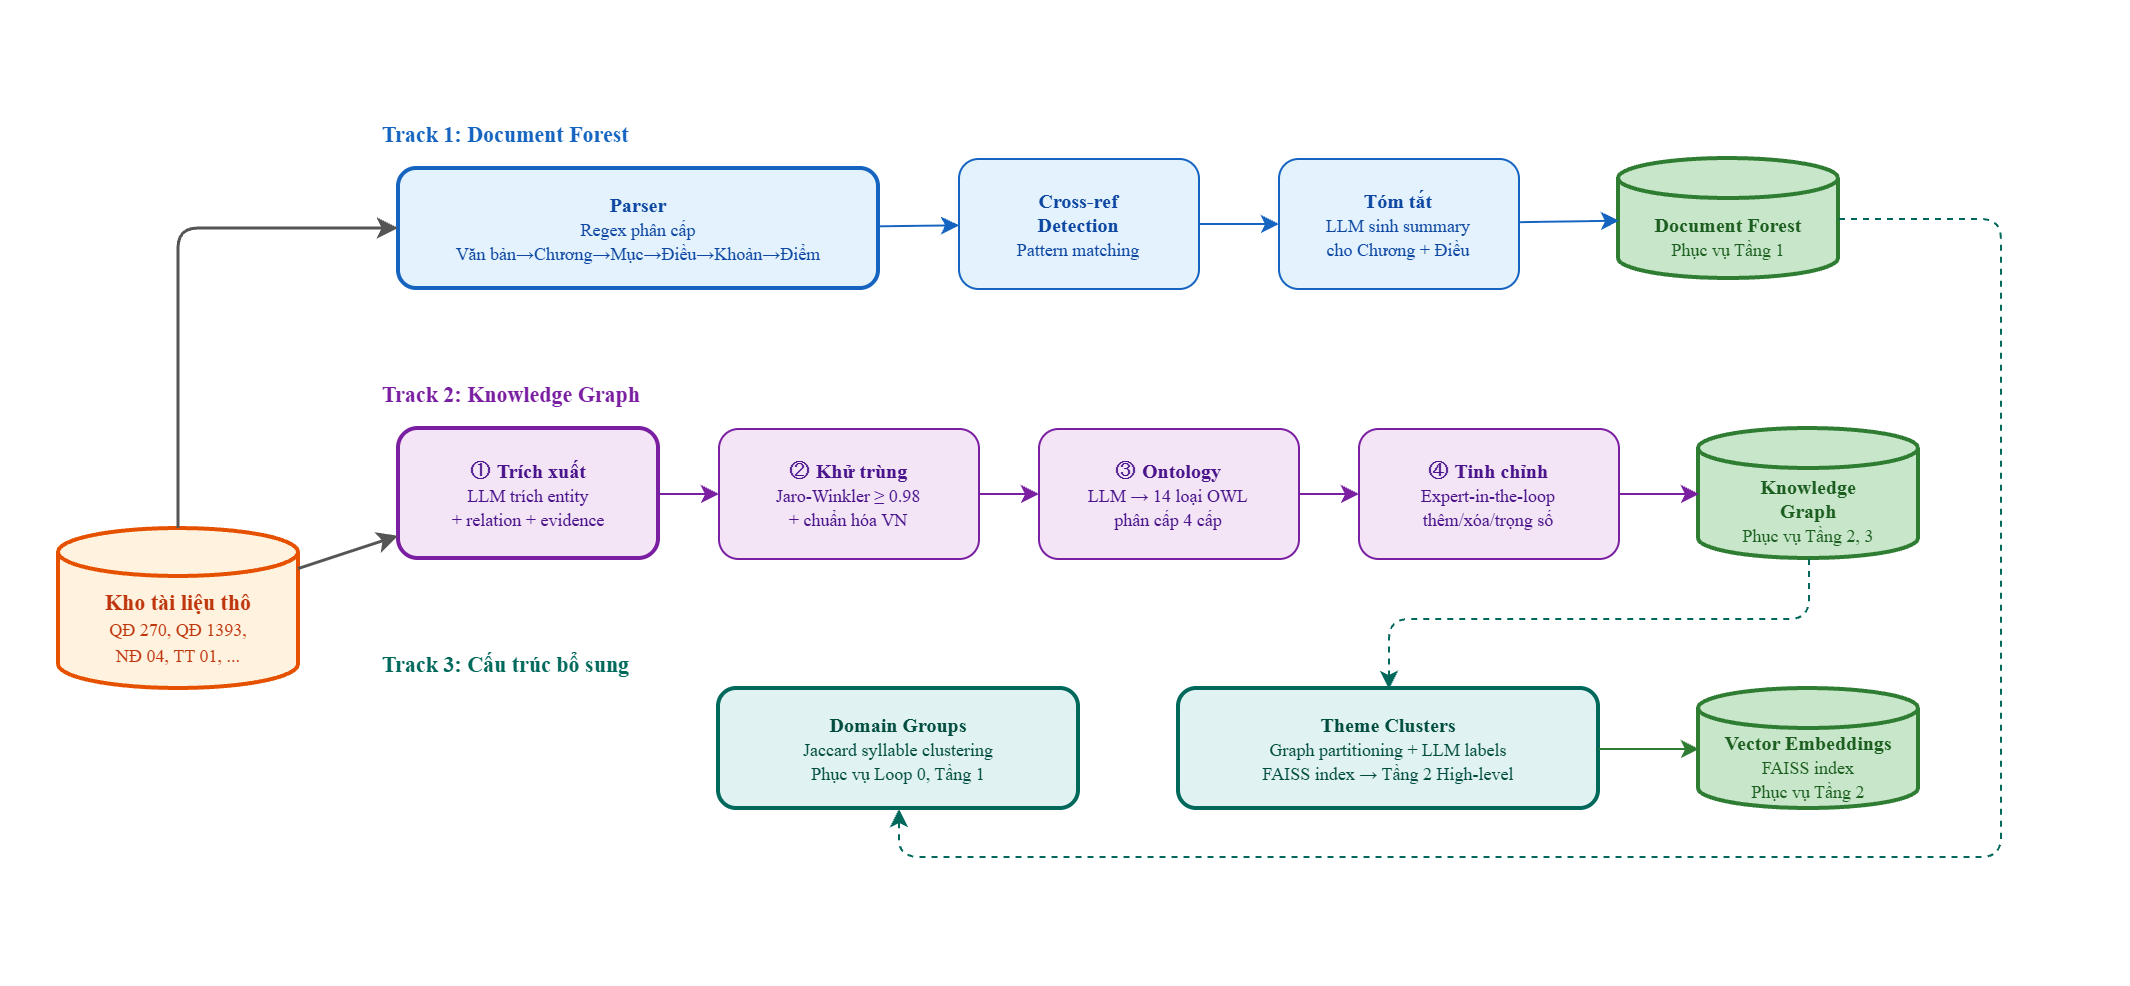
\includegraphics[width=\textwidth]{graphics/figure3-2-offline-pipeline.png}
  \caption{Quy trình xây dựng tri thức ngoại tuyến. Track 1 phân tích cấu trúc
  văn bản thành Document Forest. Track 2 xây dựng Knowledge Graph qua 4 bước.
  Track 3 tạo Domain Groups và Theme Clusters phục vụ tìm kiếm.}
  \label{fig:offline-pipeline}
\end{figure}

% -------------------------------------------------------------------
\subsection{Pha trực tuyến}
\label{subsec:pha-truc-tuyen}

Pha trực tuyến đầu tiên phân tích truy vấn (phân loại ý định, mở rộng viết tắt,
trích xuất thực thể giống), sau đó xử lý qua ba tầng truy xuất: duyệt cây hướng
dẫn bởi LLM (Tầng 1), truy xuất ngữ nghĩa hai cấp trên Knowledge Graph (Tầng 2),
và hợp nhất với mở rộng Knowledge Graph (Tầng 3).

% =====================================================================
\section{Phân tích truy vấn}
\label{sec:phan-tich-truy-van}

Trước khi đưa vào ba tầng truy xuất, truy vấn thô $q$ từ người dùng được xử lý qua
bộ phân tích truy vấn gồm ba bước: phân loại ý định, mở rộng viết tắt, và trích
xuất thực thể giống. Mỗi bước tạo ra một đầu ra cụ thể phục vụ cho các tầng truy
xuất khác nhau ở giai đoạn sau. Hình~\ref{fig:query-analysis} minh họa toàn bộ
pipeline phân tích.

\begin{figure}[htbp]
  \centering
  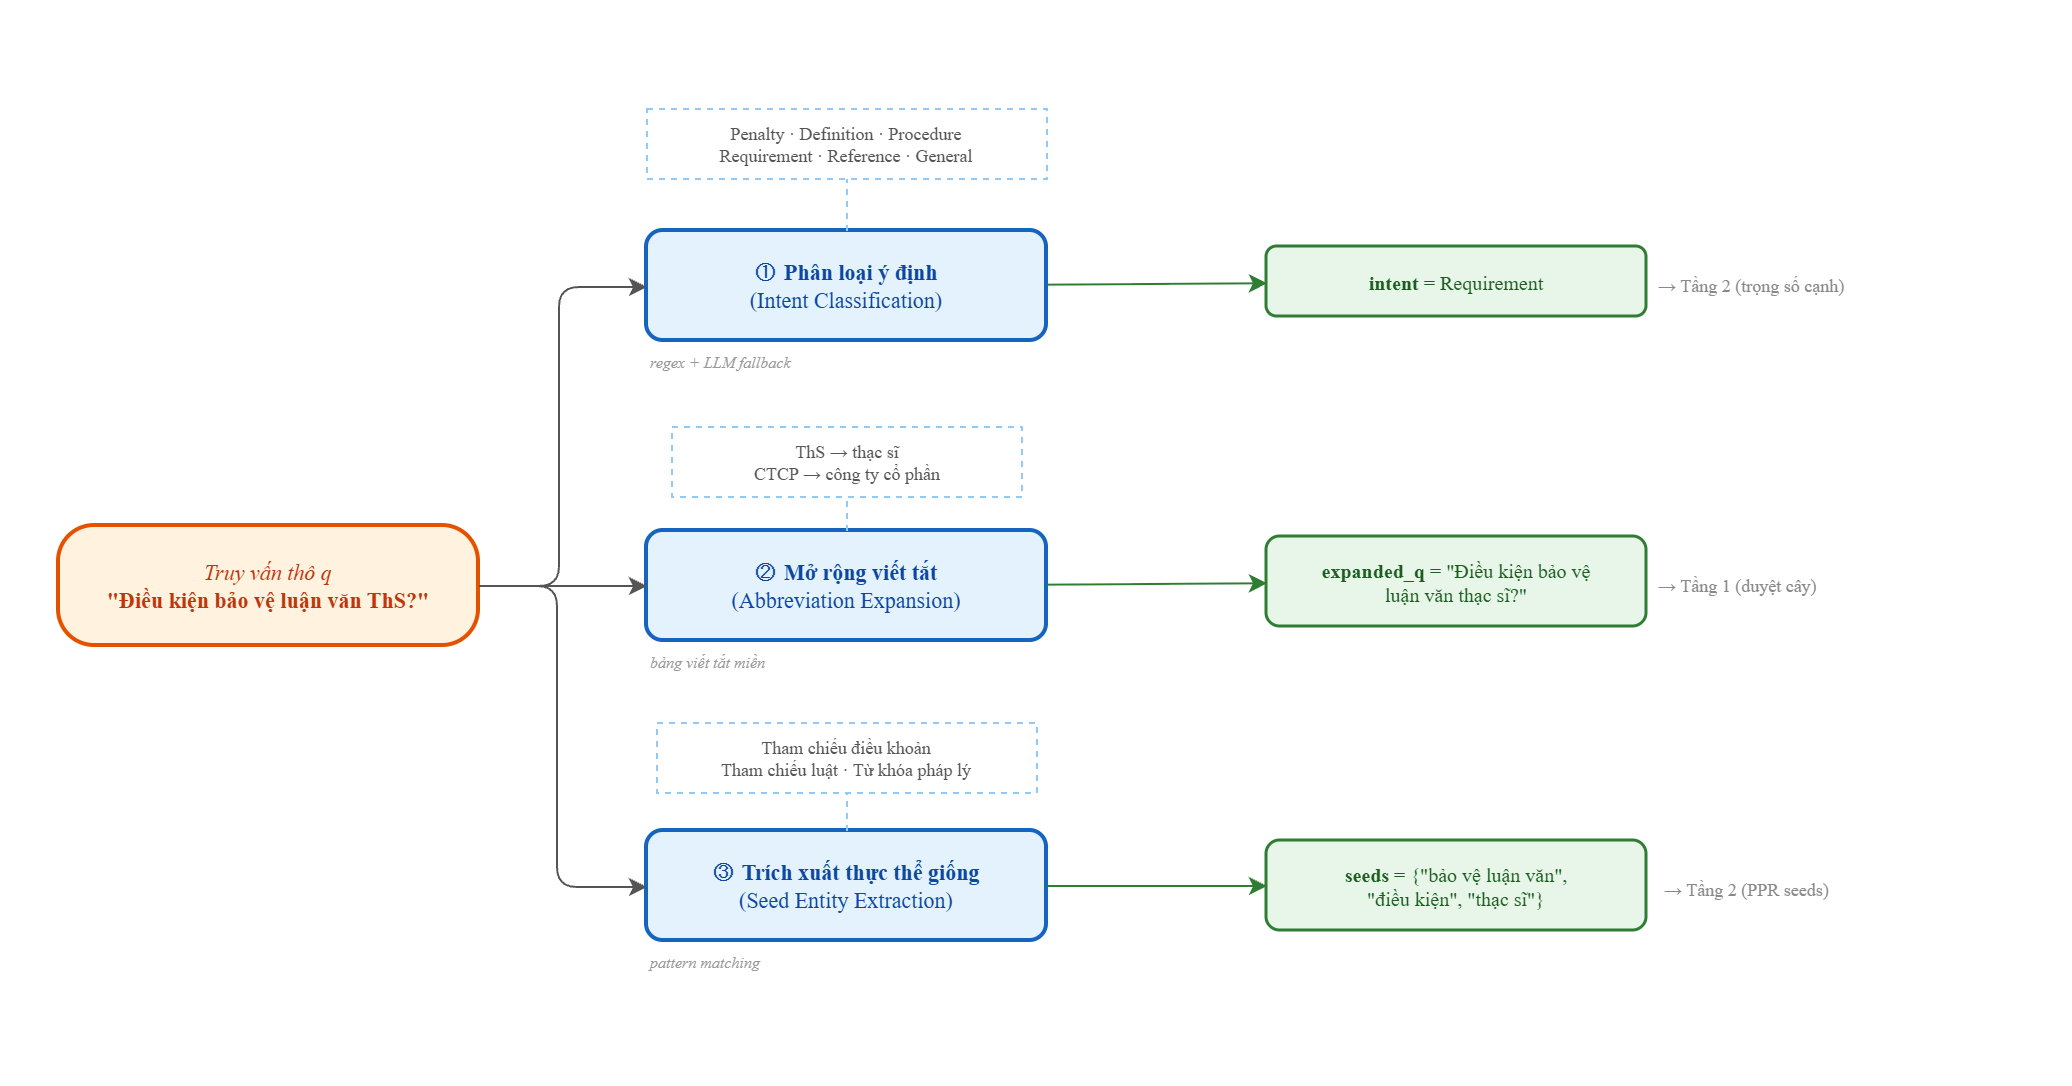
\includegraphics[width=\textwidth]{graphics/figure3-3-query-analysis.png}
  \caption{Pipeline phân tích truy vấn gồm ba bước: phân loại ý định (6 loại),
  mở rộng viết tắt, và trích xuất thực thể giống. Mỗi đầu ra phục vụ một tầng
  truy xuất khác nhau.}
  \label{fig:query-analysis}
\end{figure}

% -------------------------------------------------------------------
\subsection{Phân loại ý định}
\label{subsec:phan-loai-y-dinh}

Bước đầu tiên phân loại truy vấn thành một trong sáu loại ý định
(Bảng~\ref{tab:intent-types}), sử dụng đối sánh từ khóa tiếng Việt theo thứ tự ưu
tiên. Hệ thống duyệt tuần tự các mẫu regex: nếu truy vấn chứa từ khóa khớp với
mẫu có ưu tiên cao nhất, ý định tương ứng được gán; nếu không khớp bất kỳ mẫu nào,
ý định mặc định là GENERAL.

\begin{table}[htbp]
  \centering
  \caption{Sáu loại ý định truy vấn và mẫu nhận diện}
  \label{tab:intent-types}
  \begin{tabular}{llp{6cm}}
    \toprule
    \textbf{Ý định} & \textbf{Từ khóa tiếng Việt} & \textbf{Ví dụ truy vấn} \\
    \midrule
    Xử phạt (Penalty)
      & phạt, hình phạt, mức phạt, xử phạt
      & ``Mức phạt khi không nộp báo cáo đúng hạn?'' \\
    Định nghĩa (Definition)
      & là gì, định nghĩa, nghĩa là
      & ``Cổ đông sáng lập là gì?'' \\
    Thủ tục (Procedure)
      & thủ tục, quy trình, hồ sơ
      & ``Thủ tục bảo vệ luận văn gồm những bước nào?'' \\
    Yêu cầu (Requirement)
      & điều kiện, yêu cầu, cần phải
      & ``Điều kiện tốt nghiệp thạc sĩ tại UIT?'' \\
    Tham chiếu (Reference)
      & Điều + số (regex)
      & ``Điều 24 QĐ 270 quy định gì?'' \\
    Chung (General)
      & (mặc định)
      & ``Học viên có thể chuyển ngành được không?'' \\
    \bottomrule
  \end{tabular}
\end{table}

Nhãn ý định ảnh hưởng đến hai giai đoạn sau: thứ nhất, Tầng 2 sử dụng nhãn để điều chỉnh
trọng số cạnh trong thuật toán Personalized PageRank -- các cạnh dẫn đến thực thể
liên quan đến ý định nhận trọng số 1,0 trong khi các cạnh khác nhận 0,5; thứ hai, bước
sinh câu trả lời sử dụng nhãn để chọn prompt IRAC phù hợp -- ví dụ ý định PENALTY
hướng dẫn LLM nhấn mạnh mức phạt cụ thể và điều luật áp dụng, trong khi ý định
PROCEDURE hướng dẫn liệt kê các bước theo trình tự.

% -------------------------------------------------------------------
\subsection{Mở rộng viết tắt}
\label{subsec:mo-rong-viet-tat}

Văn bản pháp luật và quy chế đào tạo Việt Nam sử dụng phổ biến các viết tắt chuyên
ngành: CTCP (Công ty cổ phần), TNHH (Trách nhiệm hữu hạn), HĐQT (Hội đồng quản
trị), GVHD (Giáo viên hướng dẫn), v.v. Người dùng thường nhập câu hỏi với các viết
tắt này, gây khó khăn cho bước đối sánh ngữ nghĩa vì mô hình nhúng (embedding model)
không được huấn luyện trên các viết tắt đặc thù tiếng Việt.

Bộ mở rộng viết tắt sử dụng từ điển 49 mục được xây dựng thủ công, bao gồm 5 nhóm
chính (Bảng~\ref{tab:abbreviation-groups}). Thuật toán duyệt truy vấn với regex ranh
giới từ (word boundary), ưu tiên viết tắt dài hơn trước để tránh khớp nhầm (ví dụ:
``TNHH 2TV'' được khớp trước ``TNHH'').

\begin{table}[htbp]
  \centering
  \caption{Phân nhóm từ điển viết tắt (49 mục)}
  \label{tab:abbreviation-groups}
  \begin{tabular}{lcp{7cm}}
    \toprule
    \textbf{Nhóm} & \textbf{Số mục} & \textbf{Ví dụ} \\
    \midrule
    Loại hình doanh nghiệp & 5 & CTCP, TNHH, DNTN, HTX, DN \\
    Chức danh \& tổ chức   & 9 & HĐQT, HĐTV, ĐHĐCĐ, TGĐ, GĐ, BKS \\
    Văn bản pháp luật      & 4 & NĐ, TT, QĐ, NQ \\
    Đăng ký kinh doanh     & 4 & GCNĐKKD, GCNĐKDN, ĐKKD, VĐL \\
    Cơ quan nhà nước        & 6 & UBND, HĐND, CP, QH, BTC, BKHĐT \\
    Đào tạo                & 7 & GVHD, HV, NCS, ĐH, ĐHQG, ThS, TS \\
    Khác                   & 14 & MST, HKD, cty/Cty, v.v. \\
    \bottomrule
  \end{tabular}
\end{table}

Ngoài mở rộng viết tắt, hệ thống còn áp dụng bảng đồng nghĩa (synonym mapping) gồm
18 mục chuyển đổi cách diễn đạt thông dụng sang thuật ngữ pháp lý chính thức. Ví dụ:
``lập công ty'' $\to$ ``thành lập doanh nghiệp, đăng ký doanh nghiệp''; ``đóng cửa''
$\to$ ``giải thể doanh nghiệp, chấm dứt hoạt động''. Truy vấn sau khi mở rộng viết
tắt và đồng nghĩa được sử dụng trực tiếp cho Tầng 1 (duyệt cây) và tính vector nhúng
cho Tầng 2.

% -------------------------------------------------------------------
\subsection{Trích xuất thực thể giống}
\label{subsec:trich-xuat-thuc-the}

Bước cuối cùng trích xuất ba loại thực thể giống (seed entities) từ truy vấn, phục vụ
làm điểm khởi tạo cho thuật toán Personalized PageRank trong Tầng 2:

\begin{enumerate}
  \item \textbf{Tham chiếu điều khoản (Article Reference):} Nhận diện các tham chiếu
        dạng ``Điều + số'' bằng regex \texttt{[Đđ]iều\textbackslash s+(\textbackslash d+)},
        bao gồm cả dạng viết tắt ``Đ.~5''. Các điều khoản được khớp ngược với
        Document Forest để xác định nút tương ứng. Ví dụ: truy vấn ``Điều 24 QĐ 270
        quy định gì?'' trích xuất tham chiếu đến nút \texttt{270-QD-DHCNTT:d24}.

  \item \textbf{Tham chiếu văn bản luật (Law Reference):} Nhận diện số hiệu văn bản
        pháp luật theo định dạng \texttt{số/năm/cơ\_quan} bằng regex, ví dụ:
        ``Luật số 68/2014/QH13'' $\to$ \texttt{68/2014/QH13}. Tham chiếu này được
        sử dụng để thu hẹp không gian tìm kiếm trong Loop 0 của Tầng 1.

  \item \textbf{Từ khóa pháp lý (Legal Keywords):} Sau khi loại bỏ 15 từ dừng tiếng
        Việt phổ biến (là, gì, của, trong, và, các, có, được, để, cho, về, với, khi,
        này, theo) và các token chỉ chứa số, các từ còn lại có độ dài $\geq 2$ âm
        tiết được giữ lại làm từ khóa. Từ khóa được đối sánh với tên thực thể trong
        Knowledge Graph để chọn seed cho PPR.
\end{enumerate}

Bảng~\ref{tab:query-analysis-example} minh họa đầu ra đầy đủ của bộ phân tích truy
vấn trên ba câu hỏi mẫu thuộc các loại ý định khác nhau.

\begin{table}[htbp]
  \centering
  \caption{Ví dụ phân tích truy vấn trên ba câu hỏi mẫu}
  \label{tab:query-analysis-example}
  \resizebox{\textwidth}{!}{\begin{tabular}{p{4.5cm}p{1.8cm}p{3.5cm}p{4cm}}
    \toprule
    \textbf{Truy vấn gốc} & \textbf{Ý định} & \textbf{Viết tắt mở rộng} & \textbf{Thực thể giống} \\
    \midrule
    ``Mức phạt khi CTCP không nộp báo cáo tài chính?''
      & Penalty
      & CTCP $\to$ Công ty cổ phần
      & Từ khóa: [phạt, báo cáo tài chính, công ty cổ phần] \\
    \addlinespace
    ``Điều 24 QĐ 270 quy định gì về bảo vệ luận văn?''
      & Reference
      & QĐ $\to$ Quyết định
      & Điều: [24]; Từ khóa: [bảo vệ, luận văn] \\
    \addlinespace
    ``Thủ tục xin gia hạn thời gian đào tạo?''
      & Procedure
      & --
      & Từ khóa: [gia hạn, thời gian, đào tạo] \\
    \bottomrule
  \end{tabular}}
\end{table}

Các đầu ra từ bộ phân tích truy vấn được phân phối cho các tầng truy xuất như sau:
Tầng 1 nhận truy vấn đã mở rộng viết tắt để cải thiện đối sánh tóm tắt chương/điều;
Tầng 2 nhận thực thể giống làm seed cho PPR và nhãn ý định để điều chỉnh trọng số
cạnh; và Tầng 3 sử dụng tham chiếu điều khoản (nếu có) để bổ sung trực tiếp vào
danh sách ứng viên trước khi hợp nhất RRF.

% =====================================================================
\section{Pipeline truy xuất ba tầng}
\label{sec:pipeline-truy-xuat}

Ba tầng truy xuất hoạt động tuần tự trên các biểu diễn tri thức đã xây dựng: Tầng~1
khai thác cấu trúc phân cấp Document Forest, Tầng~2 khai thác cấu trúc ngữ nghĩa
Knowledge Graph, và Tầng~3 hợp nhất kết quả từ hai tầng trước với mở rộng đồ thị.

% -------------------------------------------------------------------
\subsection{Tầng 1: Duyệt cây cấu trúc hướng dẫn bởi LLM}
\label{subsec:tang1-duyet-cay}

Tầng 1 nhận truy vấn đã mở rộng và Document Forest, trả về danh sách xếp hạng
các điều khoản ứng viên với điểm cấu trúc. Lấy cảm hứng từ PageIndex
\cite{zhang2025pageindex}, Tầng 1 sử dụng suy luận LLM để duyệt cây từ trên xuống
(top-down) qua ba vòng lặp thu hẹp dần không gian tìm kiếm: từ toàn bộ kho văn
bản xuống tài liệu, rồi chương, rồi điều khoản cụ thể. Mỗi vòng lặp tạo ra một
chuỗi suy luận (reasoning trace) phục vụ khả năng giải thích (interpretability).

\textbf{Vòng lặp 0: Chọn tài liệu.}
Khi kho có nhiều hơn một tài liệu, LLM được cung cấp danh sách các nhóm miền
(domain group) cùng từ khóa đặc trưng đã tính toán trước trong giai đoạn offline.
LLM chọn nhóm miền phù hợp nhất với truy vấn, từ đó xác định tập tài liệu liên
quan. Nếu nhóm miền chứa nhiều hơn 5 tài liệu, LLM được gọi lần hai để thu hẹp
xuống tối đa 5 tài liệu dựa trên tóm tắt phạm vi (scope preview) của từng tài
liệu.

Cơ chế fallback: nếu LLM không trả về kết quả hợp lệ, hệ thống sử dụng đối sánh
từ khóa (keyword overlap) giữa các âm tiết trong truy vấn và từ khóa miền để chọn
nhóm có điểm trùng khớp cao nhất.

\textbf{Vòng lặp 1: Chọn chương.}
LLM nhận cấu trúc tài liệu gồm tên và mô tả tóm tắt của từng chương, cùng với
truy vấn (có gợi ý ngữ nghĩa từ bước mở rộng truy vấn nếu có). LLM chọn tối đa 8
chương phù hợp nhất và trả về JSON chứa danh sách index cùng độ tin cậy (xem Phụ
lục D, Bảng D.4). Nhiệt độ (temperature) $= 0{,}0$ đảm bảo kết quả xác định, loại
bỏ phương sai giữa các lần chạy.

Hai cơ chế bổ sung:
\begin{itemize}
  \item \textbf{Tự động bổ sung chương ``Quy định chung'':} Các chương chứa định
        nghĩa thuật ngữ và phạm vi áp dụng (thường là Chương 1) được tự động thêm
        vào nếu LLM chưa chọn, vì các chương này thường chứa các điều khoản nền
        tảng cần thiết để hiểu các điều khoản chuyên biệt.

  \item \textbf{Mở rộng khi độ tin cậy thấp:} Nếu LLM chỉ chọn một chương với
        độ tin cậy (confidence) $< 0{,}98$, hệ thống gọi LLM lần hai với các
        chương còn lại để xem xét bổ sung thêm, giảm rủi ro bỏ sót khi truy vấn
        mơ hồ.
\end{itemize}

Cơ chế fallback: nếu LLM thất bại, hệ thống chọn các chương có nhiều điều khoản
nhất (thay vì chọn theo thứ tự xuất hiện), vì các chương lớn thường bao phủ nhiều
chủ đề hơn.

\textbf{Vòng lặp 2: Chọn điều khoản.}
Với mỗi chương đã chọn, LLM nhận danh sách điều khoản kèm tóm tắt (tiêu đề, từ
khóa) và chọn tối đa 7 điều khoản phù hợp (xem Phụ lục D, Bảng D.5). Nhiệt độ
$= 0{,}0$ cho kết quả ổn định. Trước khi gọi LLM, hệ thống bổ sung hai tín hiệu
hỗ trợ vào thông tin mỗi điều khoản:

\begin{itemize}
  \item \textbf{Điểm ngữ nghĩa (semantic score):} Cosine similarity giữa vector
        nhúng truy vấn và vector nhúng của tiêu đề + từ khóa điều khoản, chuyển
        thành thứ hạng tương đối (semantic\_rank, 1 = phù hợp nhất).

  \item \textbf{Điểm KG (dual score):} Điểm từ Tầng 2 (DualLevel Retriever) chạy
        ở chế độ low-level, chuyển thành thứ hạng tương đối (dual\_rank). Tín hiệu
        này giúp LLM ưu tiên các điều khoản có liên kết KG mạnh với truy vấn.
\end{itemize}

Prompt hướng dẫn LLM ưu tiên các điều khoản có thứ hạng thấp (rank thấp = phù
hợp hơn), nhưng LLM vẫn có quyền quyết định cuối cùng dựa trên nội dung tóm tắt.

Sau khi tất cả chương được xử lý, các điều khoản được gộp, loại trùng lặp, và giới
hạn tổng số lượng. Điểm tin cậy tổng hợp của Tầng 1 được tính bằng trung bình có
trọng số giữa confidence của Loop 1 ($\times 0{,}45$) và trung bình confidence của
Loop 2 ($\times 0{,}55$), giới hạn tối đa $0{,}95$.

Logic retry (3 lần, exponential backoff) được áp dụng cho tất cả lời gọi LLM để
xử lý các lỗi tạm thời từ proxy hoặc API.

Hình~\ref{fig:tree-traversal} minh họa quá trình duyệt cây ba vòng lặp với một
truy vấn ví dụ từ miền quy định đào tạo.

\begin{figure}[htbp]
  \centering
  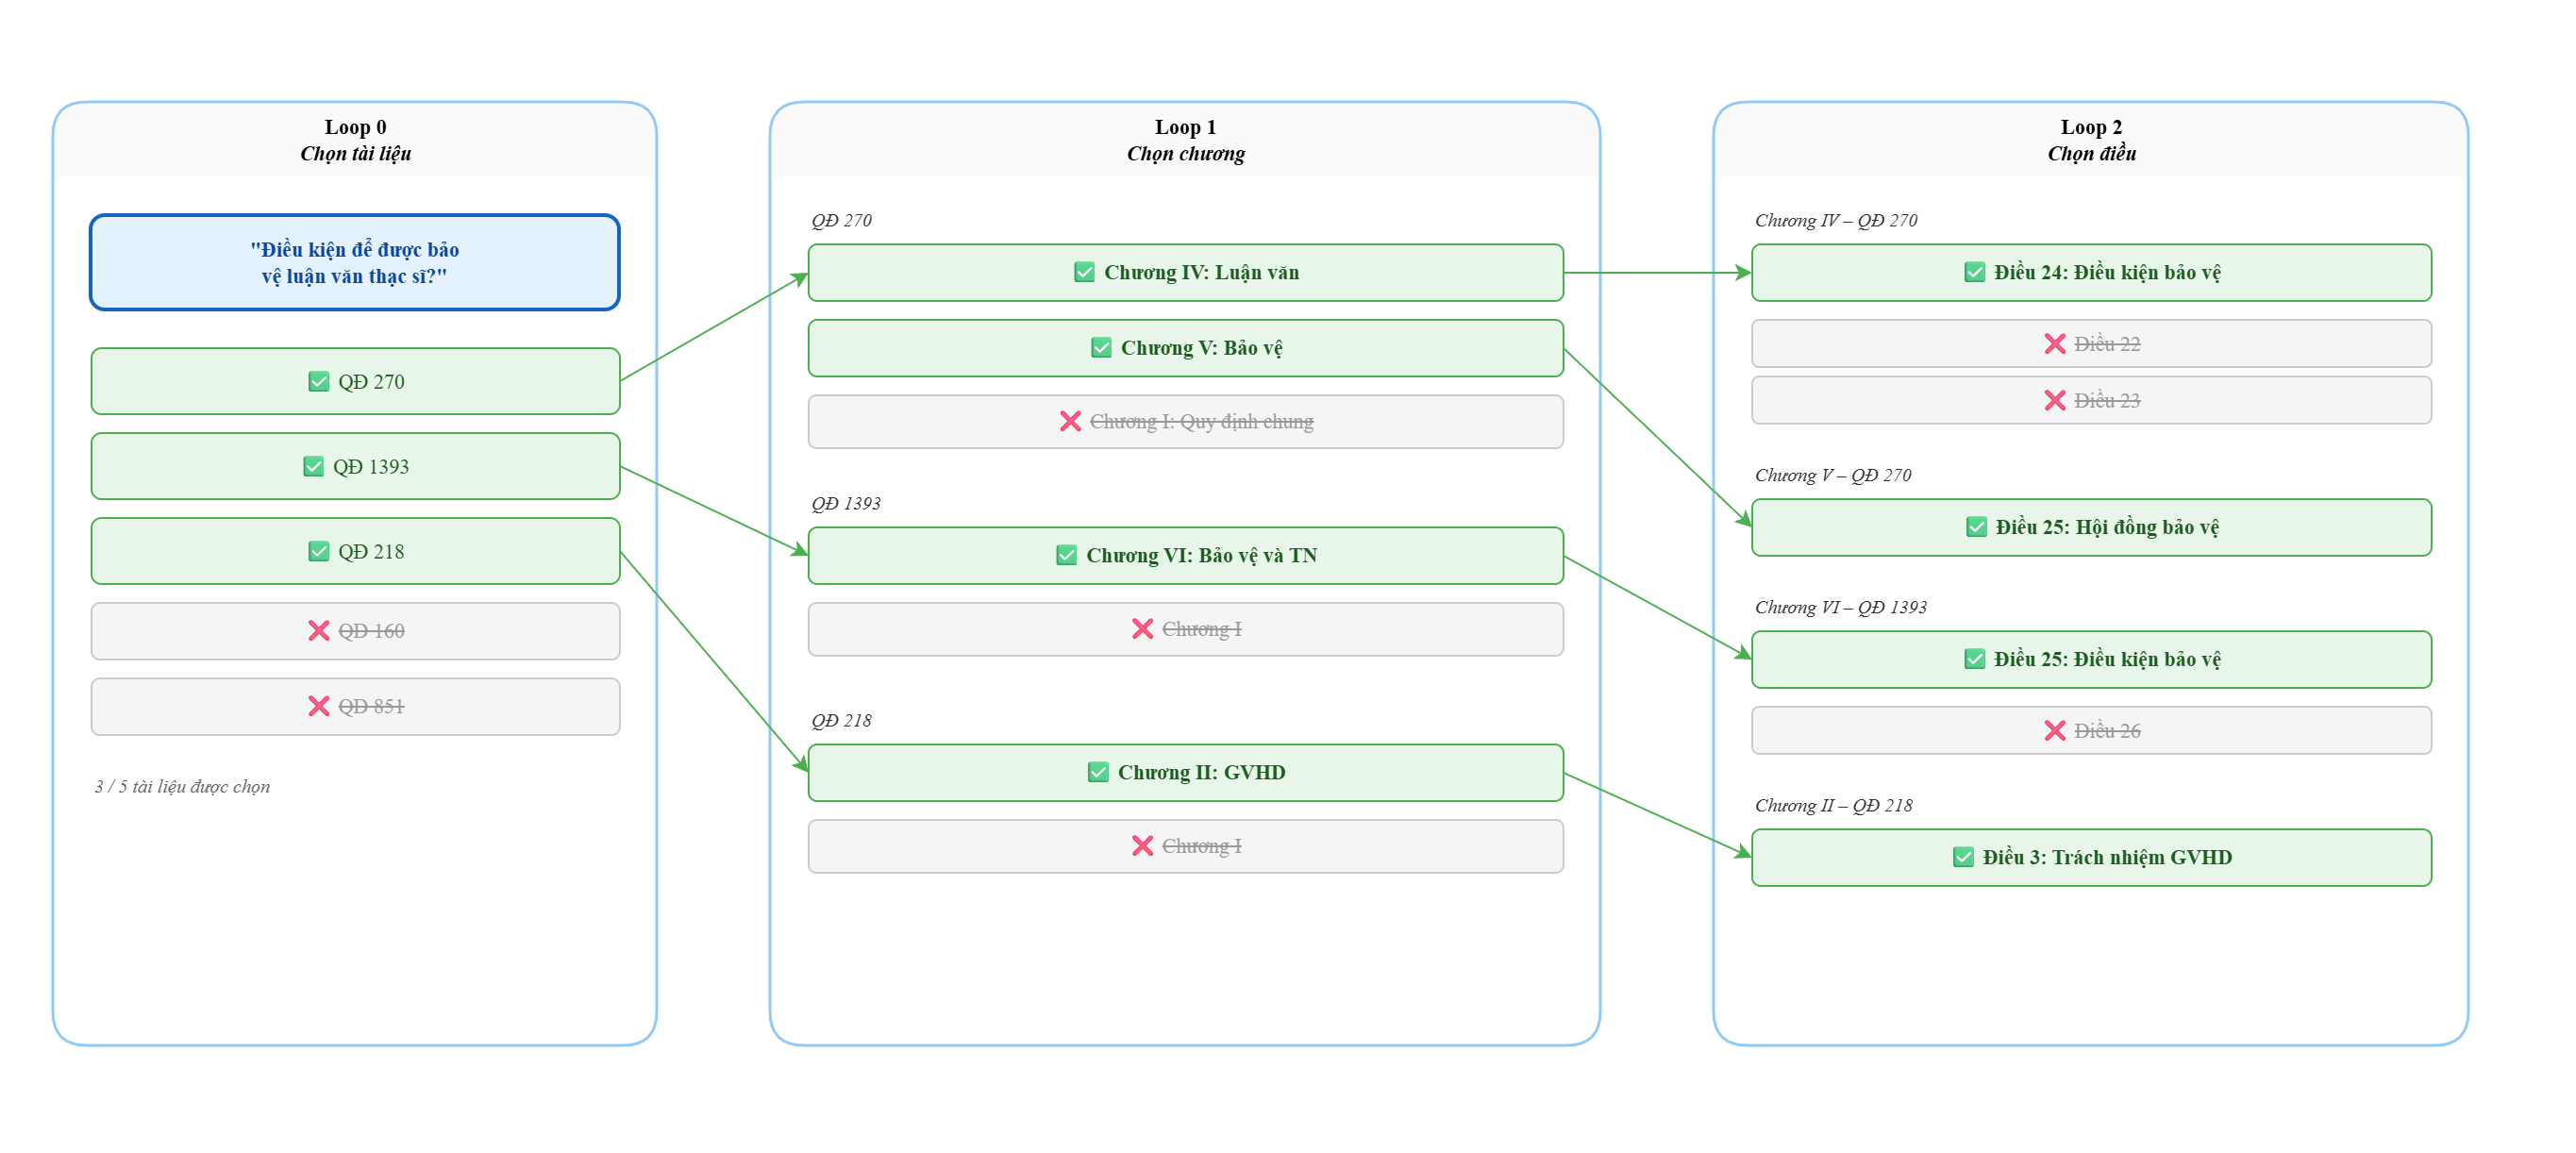
\includegraphics[width=\textwidth]{graphics/figure3-4-tree-traversal.png}
  \caption{Minh họa quá trình duyệt cây ba vòng lặp với truy vấn ``Điều kiện để
  được bảo vệ luận văn thạc sĩ?''. Các nút xanh là được chọn bởi LLM, các nút
  xám bị loại. Loop 0 chọn 3/5 tài liệu, Loop 1 thu hẹp xuống các chương liên
  quan, Loop 2 xác định các điều khoản cụ thể.}
  \label{fig:tree-traversal}
\end{figure}

% -------------------------------------------------------------------
\subsection{Tầng 2: Truy xuất ngữ nghĩa hai cấp}
\label{subsec:tang2-semantic}

Tầng 2 nhận các thực thể đã trích xuất và nhãn ý định từ bước phân tích truy vấn
(Mục~\ref{sec:phan-tich-truy-van}), kết hợp với Knowledge Graph để tính điểm ngữ
nghĩa cho từng điều khoản. Khác với Tầng 1 sử dụng LLM để duyệt cây top-down,
Tầng 2 tiếp cận bottom-up: xuất phát từ các thực thể trong KG, lan truyền điểm số
qua các quan hệ ontology để tìm các điều khoản liên quan. Tầng này hoạt động ở hai
cấp: low-level (entity-specific) tập trung vào từng thực thể cụ thể, và high-level
(conceptual) nắm bắt mối liên hệ chủ đề giữa các cụm khái niệm.

\subsubsection{Low-level (Entity-specific)}
\label{subsubsec:low-level}

Low-level tính bốn tín hiệu độc lập cho mỗi điều khoản, mỗi tín hiệu nắm bắt một
khía cạnh khác nhau của mức độ liên quan:

\subsubsection*{1. Keyphrase Matching}

So khớp các thuật ngữ trong truy vấn với tên thực thể KG bằng cách tạo n-gram âm
tiết (unigram, bigram, trigram) từ truy vấn. Với mỗi thực thể, điểm cơ bản được
tính bằng tỷ lệ trùng khớp âm tiết ($|Q \cap E| / |Q|$), sau đó được tăng cường
bởi các hệ số nhân: $\times 1{,}5$ khi trùng khớp $\geq 2$ âm tiết hoặc khi khớp
cụm bigram/trigram, $\times 1{,}5$ khi tên thực thể xuất hiện trong truy vấn
(exact match), $\times 1{,}2$ khi truy vấn là chuỗi con của tên thực thể. Điểm
keyphrase cấp điều khoản được tổng hợp từ tất cả thực thể thuộc điều khoản đó:

\begin{equation}
  s_\text{kp}(a) = \max_{e \in E_a} s(e) + 0{,}3 \cdot \ln(n+1) \cdot \bar{s}
  \label{eq:keyphrase-score}
\end{equation}

\noindent trong đó $E_a$ là tập thực thể thuộc điều khoản $a$, $n$ là số thực thể
có điểm dương, và $\bar{s}$ là điểm trung bình. Thành phần logarithmic khuyến
khích các điều khoản chứa nhiều thực thể liên quan mà không để số lượng lớn áp
đảo chất lượng khớp cao nhất.

\subsubsection*{2. Semantic Similarity}

Tính cosine similarity giữa vector nhúng (embedding) của truy vấn và vector nhúng
của từng điều khoản, sử dụng mô hình sentence-transformers MiniLM-L12-v2. Tín hiệu
này bổ sung cho đối sánh từ khóa bằng cách nắm bắt sự tương đồng ngữ nghĩa ngay
cả khi thuật ngữ không trùng khớp chính xác, ví dụ ``hủy bỏ nghị quyết'' và ``vô
hiệu quyết định'' có thể có điểm keyphrase thấp nhưng điểm semantic cao.

\subsubsection*{3. Intent-aware PPR}

Sử dụng thuật toán Personalized PageRank \cite{haveliwala2002ppr} để lan truyền
điểm số qua cấu trúc đồ thị KG. Quá trình gồm ba bước:

\begin{enumerate}[a)]
  \item Chọn các thực thể hạt giống (seed): chỉ những thực thể có điểm keyphrase
        $\geq 0{,}3$ được chọn làm seed, đảm bảo chỉ các thực thể liên quan cao
        mới khởi tạo quá trình lan truyền.

  \item Tính vector nhúng truy vấn để điều chỉnh trọng số cạnh theo ý định: các
        cạnh dẫn đến thực thể có embedding gần với truy vấn được tăng trọng số.

  \item Thực hiện PPR với công thức:
\end{enumerate}

\begin{equation}
  \text{PPR}(v) = (1 - \alpha) \sum_{u \in \mathcal{N}(v)}
                  \frac{w(u,v) \cdot \text{PPR}(u)}{d(u)}
                  + \alpha \cdot p(v)
  \label{eq:ppr}
\end{equation}

\noindent trong đó $\alpha = 0{,}15$ là xác suất teleport, $w(u,v)$ là trọng số
cạnh điều chỉnh theo ý định truy vấn, $d(u)$ là bậc ra có trọng số, và $p(v)$ là
vector cá nhân hóa (phân bố đều trên các seed). Điểm PPR cấp thực thể được quy về
cấp điều khoản bằng cách lấy giá trị lớn nhất trong các thực thể thuộc điều khoản.
Ưu điểm của PPR là phát hiện các điều khoản liên quan gián tiếp qua nhiều bước
nhảy (multi-hop) trong đồ thị, ví dụ từ thực thể ``học phí'' qua cạnh requires đến
``nghĩa vụ tài chính'' rồi đến ``chế tài vi phạm''.

\subsubsection*{4. Concept Matching}

Mở rộng kết quả keyphrase ở mức lớp ontology. Đầu tiên, thu thập các loại thực
thể (entity type) từ tất cả thực thể đã khớp keyphrase, mỗi loại được gán trọng
số bằng điểm keyphrase cao nhất của các thực thể thuộc loại đó. Sau đó, duyệt tất
cả điều khoản trong KG: với mỗi điều khoản, tính tổng trọng số các loại thực thể
trùng khớp, chia cho tổng số thực thể của điều khoản để chuẩn hóa:

\begin{equation}
  s_\text{con}(a) = \min\!\left(1,\;
    \frac{\displaystyle\sum_{e \in E_a} w_\text{type}\!\left(\text{type}(e)\right)}
         {|E_a|}
  \right)
  \label{eq:concept-score}
\end{equation}

Cơ chế này cho phép phát hiện các điều khoản có cùng loại thực thể nhưng dùng tên
gọi khác, ví dụ keyphrase khớp với thực thể ``cổ đông sáng lập'' (loại CHỦ\_THỂ)
sẽ lan truyền điểm đến các điều khoản chứa ``thành viên hợp danh'' cùng loại
CHỦ\_THỂ.

\subsubsection*{Tổng hợp điểm Low-level}

Bốn tín hiệu được kết hợp bằng tổng có trọng số ($w_\text{kp} = 0{,}05$,
$w_\text{sem} = 0{,}20$, $w_\text{ppr} = 0{,}25$, $w_\text{con} = 0{,}20$) và
chuẩn hóa về $[0, 1]$ bằng cách chia cho giá trị lớn nhất. Trọng số thấp của
keyphrase (0,05) phản ánh vai trò ``kích hoạt'' của nó: keyphrase chủ yếu cung
cấp seed cho PPR và loại thực thể cho concept matching, thay vì trực tiếp quyết
định xếp hạng. PPR nhận trọng số cao nhất (0,25) vì khả năng nắm bắt quan hệ cấu
trúc đồ thị.

\subsubsection{High-level (Conceptual)}
\label{subsubsec:high-level}

High-level hoạt động ở cấp độ trừu tượng hơn, tìm kiếm các điều khoản liên quan
thông qua cụm chủ đề (theme cluster) thay vì từng thực thể riêng lẻ.

\subsubsection*{1. Theme Matching}

Trong giai đoạn offline, các thực thể KG được nhóm thành các cụm chủ đề dựa trên
embedding similarity (ví dụ: cụm ``quản trị công ty'' gồm các thực thể về cổ đông,
hội đồng quản trị, ban kiểm soát). Mỗi cụm được biểu diễn bởi vector nhúng trung
bình. Tại thời điểm truy vấn, vector nhúng truy vấn được so khớp với top-10 cụm
chủ đề gần nhất. Từ mỗi cụm khớp, các thực thể nguồn (source entities) được truy
ngược về điều khoản chứa chúng, gán điểm theme bằng cosine similarity giữa truy
vấn và cụm.

\subsubsection*{2. Hierarchy Expansion}

Từ các điều khoản đã tìm được qua theme matching, thu thập các loại thực thể
(entity type) và tìm thêm các điều khoản khác chứa cùng loại thực thể nhưng chưa
xuất hiện trong kết quả theme. Hệ số suy giảm $0{,}5$ được áp dụng cho các điều
khoản mở rộng này để đảm bảo chúng xếp hạng thấp hơn kết quả theme trực tiếp. Ví
dụ: nếu theme matching tìm được điều khoản về ``xử phạt vi phạm'' (chứa thực thể
loại CHẾ\_TÀI), hierarchy expansion sẽ bổ sung các điều khoản khác cũng chứa thực
thể loại CHẾ\_TÀI với điểm giảm một nửa.

\subsubsection{Hợp nhất Low-level và High-level}
\label{subsubsec:merge-levels}

Hai cấp được hợp nhất bằng tổng có trọng số:

\begin{equation}
  s(a) = 0{,}70 \cdot s_\text{low}(a)
        + 0{,}15 \cdot s_\text{theme}(a)
        + 0{,}15 \cdot s_\text{hier}(a)
  \label{eq:tier2-final-score}
\end{equation}

Tỷ lệ 70--30 giữa low-level và high-level phản ánh độ tin cậy cao hơn của các tín
hiệu entity-specific (keyphrase, PPR, concept) so với tín hiệu chủ đề trừu tượng.
Các điều khoản có điểm tổng hợp dưới ngưỡng $0{,}1$ bị loại bỏ để giảm nhiễu
trước khi chuyển sang Tầng 3. Hình~\ref{fig:tier2-dual-level} minh họa kiến trúc
hai cấp của Tầng 2 với sáu tín hiệu và cách hợp nhất.

\begin{figure}[htbp]
  \centering
  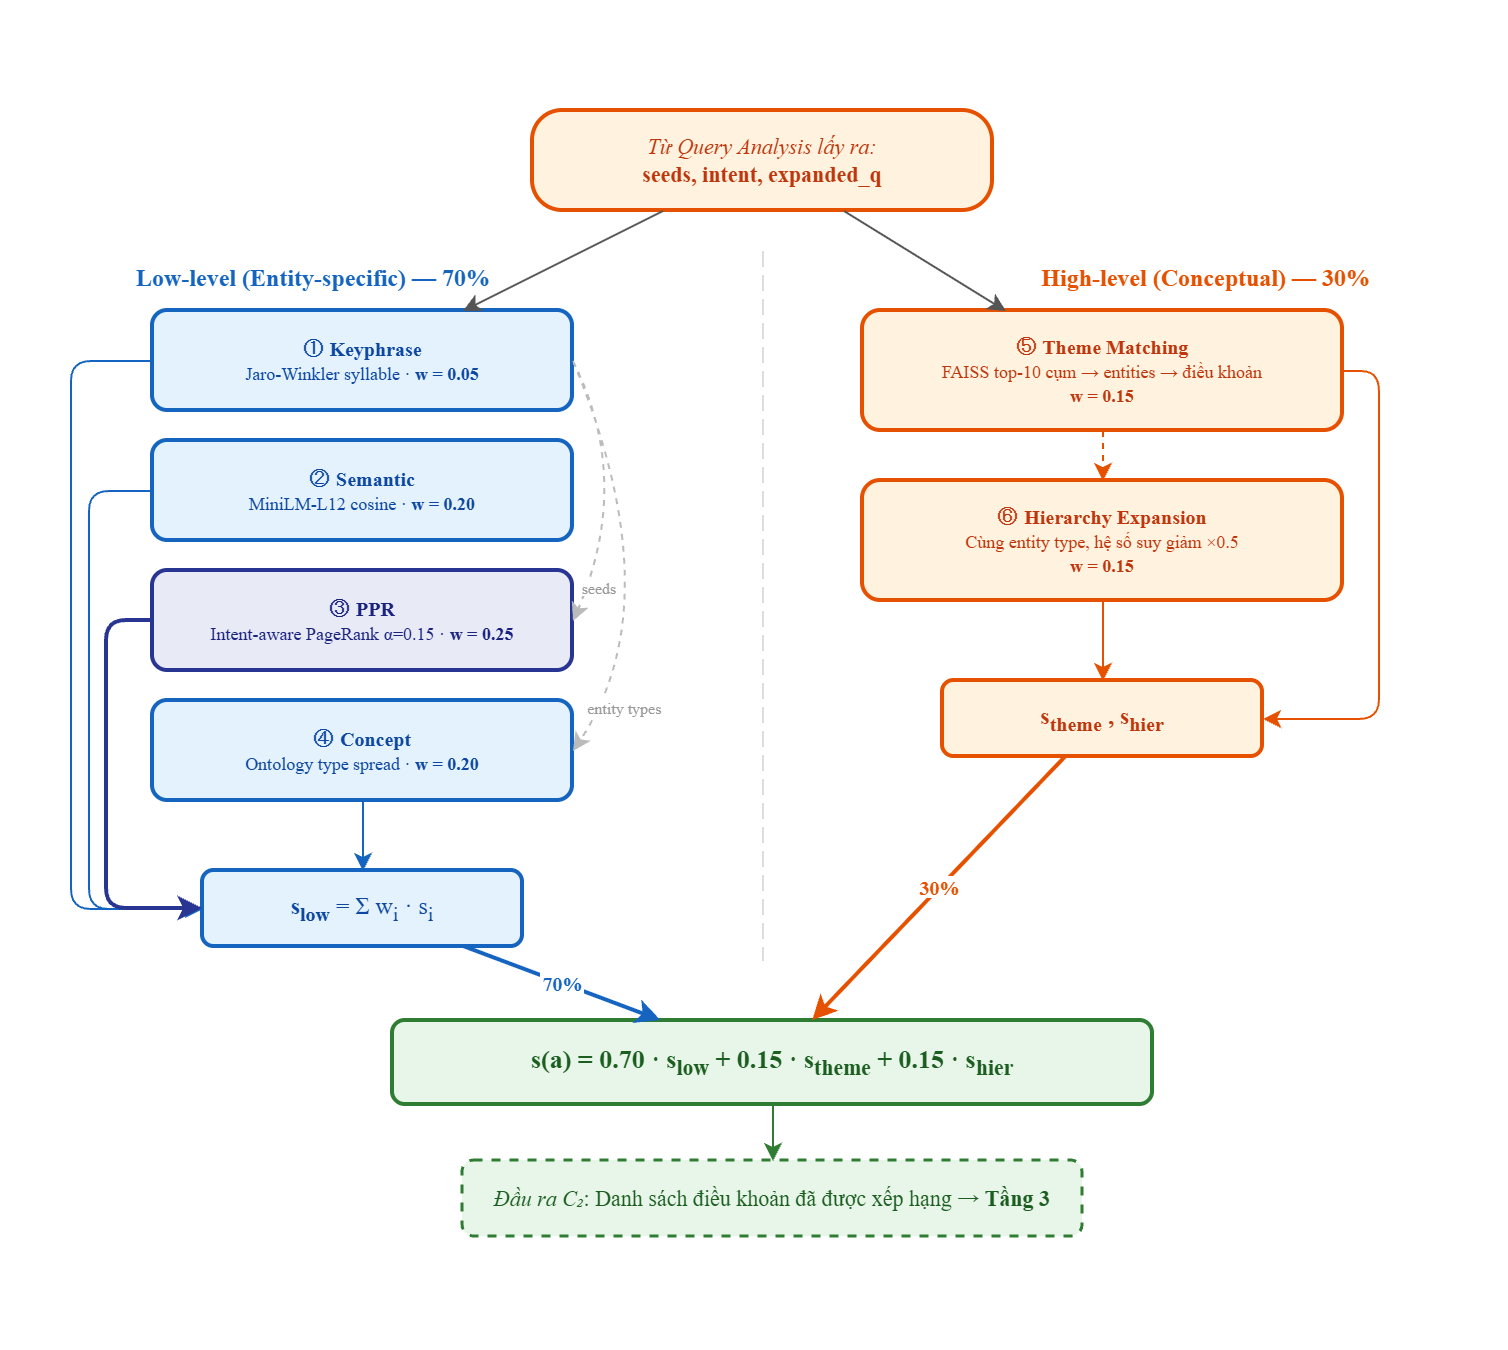
\includegraphics[width=\textwidth]{graphics/figure3-5-tier2-dual-level.png}
  \caption{Kiến trúc Tầng 2 hai cấp. Low-level gồm 4 tín hiệu (Keyphrase,
  Semantic, Intent-aware PPR, Concept Matching) với minh họa PPR lan truyền qua
  KG. High-level gồm Theme Matching và Hierarchy Expansion. Công thức hợp nhất
  70\%--30\% ưu tiên tín hiệu entity-specific.}
  \label{fig:tier2-dual-level}
\end{figure}

% -------------------------------------------------------------------
\subsection{Tầng 3: Hợp nhất RRF với mở rộng Knowledge Graph}
\label{subsec:tang3-rrf}

Tầng 3 tạo ra danh sách top-$k$ điều khoản cuối cùng thông qua ba bước: mở rộng
Knowledge Graph, RRF, và các cơ chế điều chỉnh.

\subsubsection{Mở rộng Knowledge Graph}
\label{subsubsec:kg-expansion}

Các điều khoản hạt giống từ Tầng 1 và Tầng 2 được mở rộng thông qua các cạnh quan
hệ của Knowledge Graph. Hai nhóm quan hệ được sử dụng. Nhóm quan hệ mạnh (STRONG)
gồm references, requires, depends\_on, implements, ưu tiên cho liên kết xuyên
chương. Nhóm quan hệ mở rộng (EXPANSION) gồm defined\_as, condition\_for,
related\_to, includes, bổ sung các điều khoản liên quan cùng chương. Giới hạn mở
rộng:

\begin{itemize}
  \item Khác chương (cross-chapter): tối đa 5 điều khoản.
  \item Cùng chương (same-chapter): tối đa 2 điều khoản.
\end{itemize}

Bộ lọc liên quan ngữ nghĩa (cosine similarity $\geq 0{,}4$) được áp dụng để loại
bỏ nhiễu. Kết quả mở rộng tạo thành danh sách xếp hạng thứ ba bên cạnh Tầng 1 và
Tầng 2.

\subsubsection{Reciprocal Rank Fusion}
\label{subsubsec:rrf}

Ba danh sách được hợp nhất sử dụng Reciprocal Rank Fusion \cite{cormack2009rrf}:

\begin{equation}
  \text{RRF}(d) = \sum_{s \in \{T_1,\, T_2,\, \text{KG}\}}
                  w_s \cdot \frac{1}{k + \text{rank}_s(d)}
  \label{eq:rrf}
\end{equation}

\noindent trong đó $k = 60$ và trọng số nguồn $w_{T_1} = 1{,}2$,
$w_{T_2} = 0{,}7$, $w_\text{KG} = 1{,}0$ được thiết lập thực nghiệm trên tập phát
triển và chia sẻ trên tất cả các miền. Duyệt cây nhận trọng số cao nhất vì cung
cấp tín hiệu cấu trúc đáng tin cậy nhất.

\begin{figure}[htbp]
  \centering
  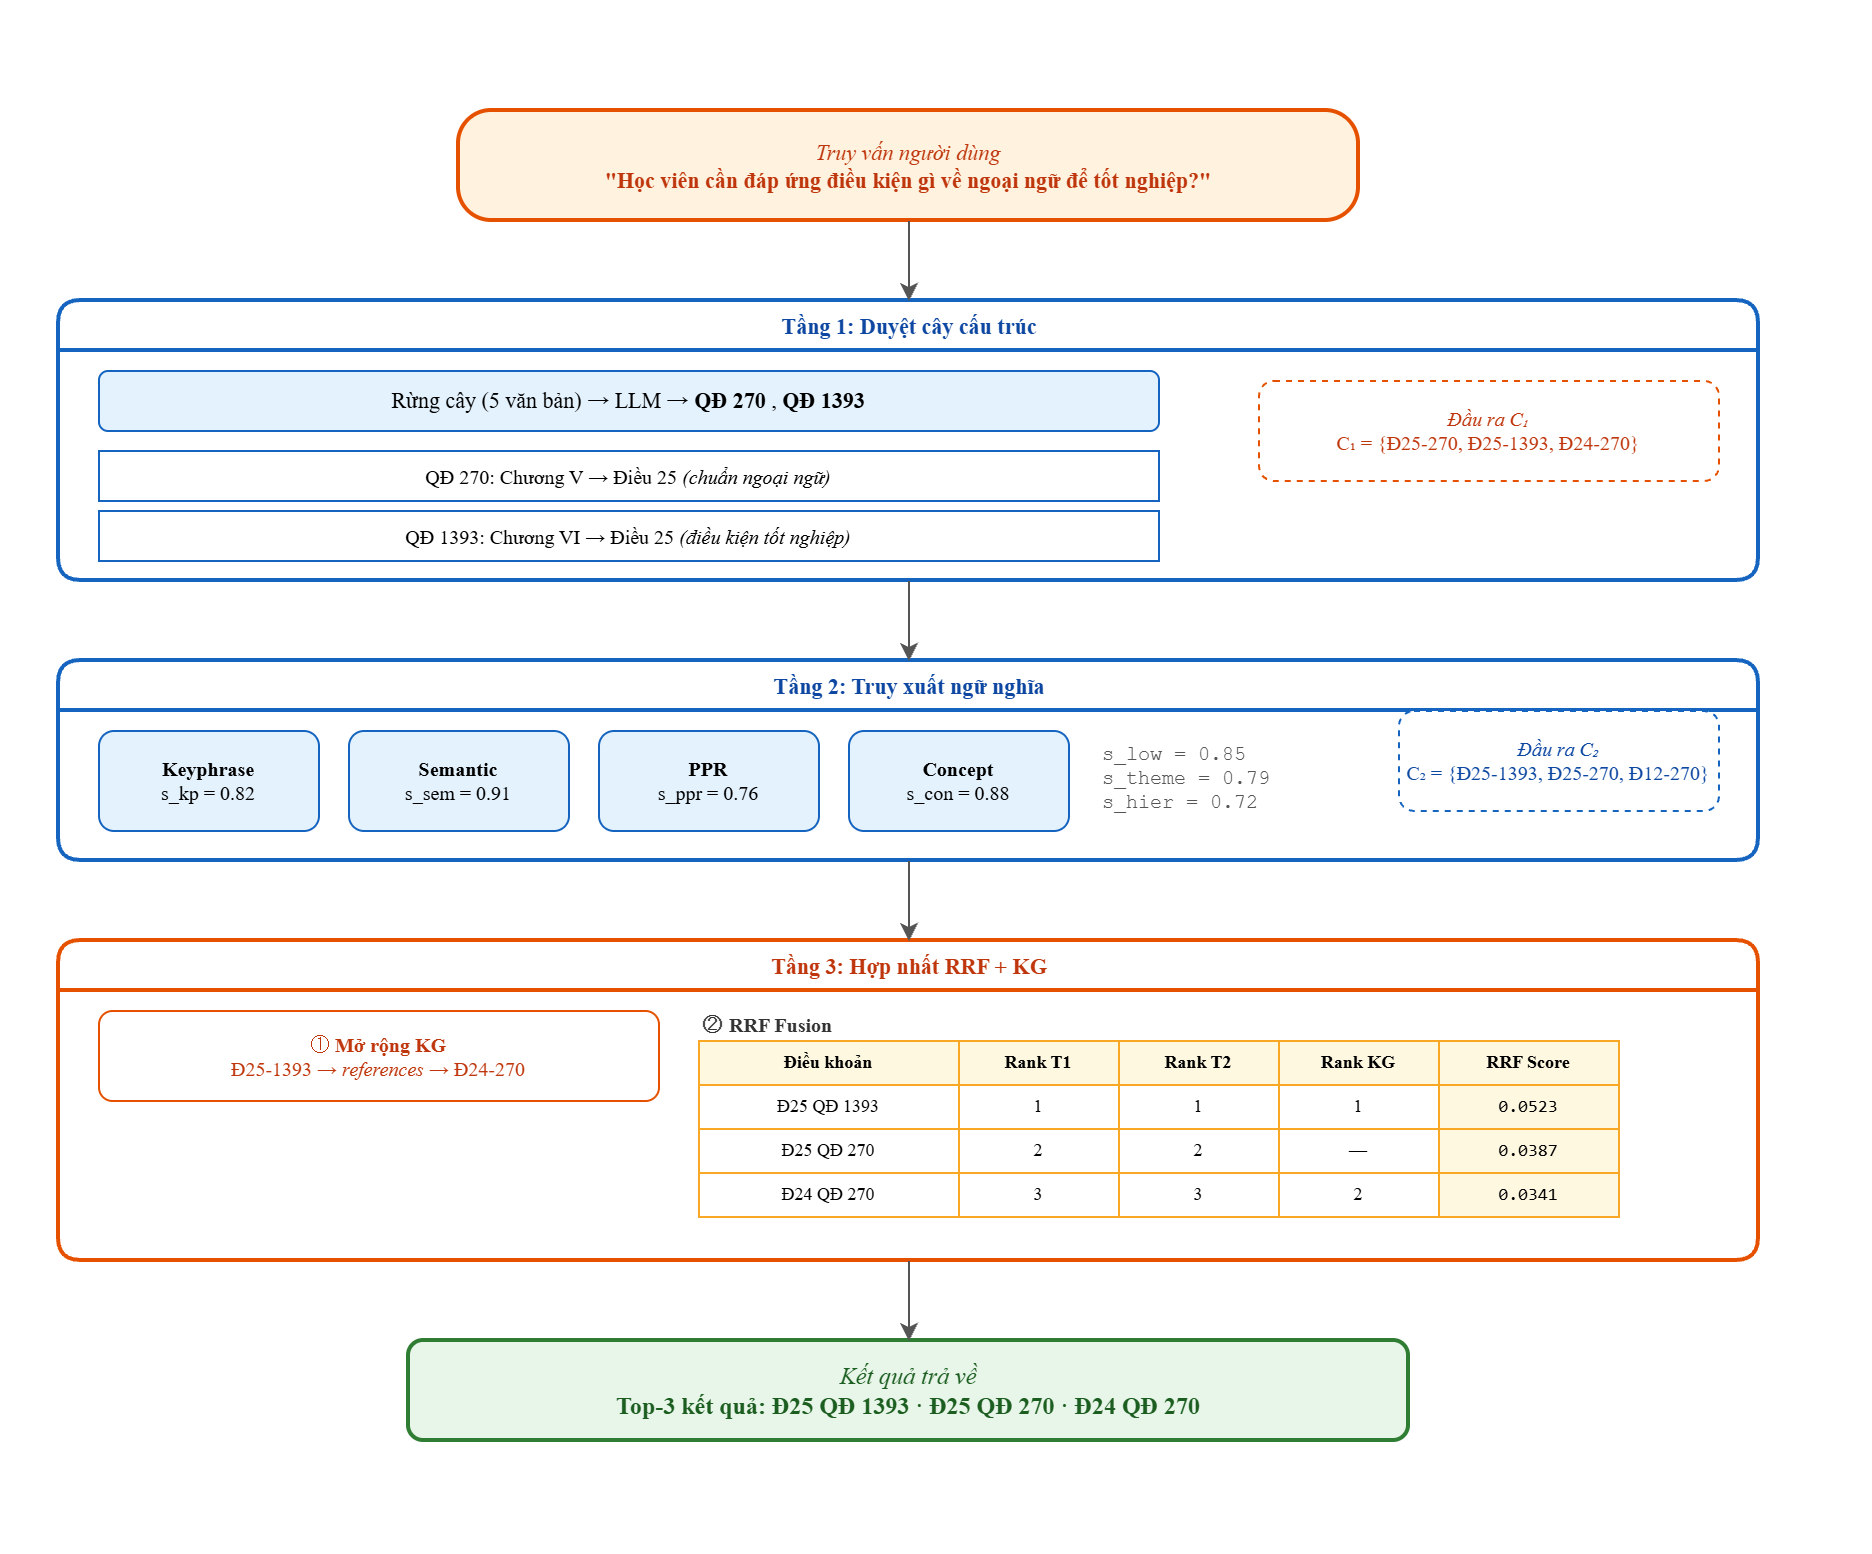
\includegraphics[width=\textwidth]{graphics/figure3-6-end-to-end-flow.png}
  \caption{Minh họa luồng xử lý end-to-end với truy vấn ``Học viên cần đáp ứng
  điều kiện gì về ngoại ngữ để tốt nghiệp?''. Tầng 1 tìm Đ.29, Đ.25, Đ.24 qua
  duyệt cây. Tầng 2 xác nhận Đ.25 và Đ.29 qua PPR, bổ sung Đ.8. Tầng 3 nhận
  seeds từ Tầng 1 và Tầng 2, mở rộng KG thêm Đ.5, sau đó hợp nhất RRF cả ba danh
  sách với thưởng đồng thuận và hệ số phạt.}
  \label{fig:end-to-end-flow}
\end{figure}

\subsubsection{Các cơ chế điều chỉnh}
\label{subsubsec:dieu-chinh}

Hệ thống áp dụng ba cơ chế điều chỉnh điểm sau hợp nhất RRF:

\begin{enumerate}
  \item \textbf{Trọng số cây động (Dynamic Tree Weight):} Khi $\geq 50\%$ điều
        khoản từ duyệt cây là điều khoản chung (generic, penalty $\leq 0{,}25$),
        trọng số cây giảm từ $1{,}2$ xuống $0{,}7$ và trọng số KG tăng từ $1{,}0$
        lên $1{,}3$.

  \item \textbf{Hệ số phạt (Penalty):}
        \begin{itemize}
          \item Procedural penalty ($0{,}35\times$): Các điều khoản thủ tục/tổ
                chức ít liên quan đến câu hỏi nội dung.
          \item Noise penalty ($0{,}35\times$): Các điều khoản có tỷ lệ đúng 0\%
                trong benchmark.
          \item Generic penalty ($0{,}15\times$): Các điều khoản phạm vi/định
                nghĩa chung (d1--d3).
        \end{itemize}

  \item \textbf{Thưởng đồng thuận (Agreement Bonus):} Điều khoản xuất hiện trong
        $\geq 2$ tầng nhận thưởng $+0{,}005$ cho mỗi tầng bổ sung, tăng cường tín
        hiệu đồng thuận xuyên tầng.

  \item \textbf{Mở rộng điều khoản lân cận (Adjacent Expansion):} Sau khi hợp nhất
        RRF, hệ thống bổ sung các điều khoản lân cận ($\pm 2$) từ mỗi kết quả, với
        điểm giảm dần theo khoảng cách. Cơ chế này khai thác quan sát rằng câu trả
        lời đúng thường nằm trong các điều khoản liền kề với kết quả truy xuất.
\end{enumerate}

Danh sách xếp hạng cuối cùng được truyền cho LLM để sinh câu trả lời có trích dẫn
nguồn.

Hình~\ref{fig:end-to-end-flow} minh họa toàn bộ luồng xử lý qua ba tầng với một
truy vấn ví dụ, thể hiện cách các tầng bổ sung lẫn nhau để tìm ra các điều khoản
liên quan.
